\section{Results}\label{sec.results}

We have implemented our prostate cancer progression model in the dReach's modeling language. The model files are available at \verb#http://www.cs.cmu.edu/~liubing/hscc15/#. All the experiments reported below were done using a machine with two Intel Xeon E5-2650 2.00GHz processors and 32GB RAM. The precision $\delta$ was set to $10^{-4}$. 

\subsection{CRC proliferation dynamics}
Due to the lack of biomarkers distinguishing HSCs and CRCs \textit{in vivo}, the proliferation kinetics of CRCs in response to androgen is far from known. Three hypotheses, denoted as $H_1$, $H_2$ and $H_3$ have been proposed to describe the androgen-depenent CRC growth  \cite{ideta08}, which are discriminated by the value of $d$ in our model, i.e.:
\begin{itemize}
\item $H_1: d = 0$, the grow of CRCs is independent of $z(t)$;
\item $H_2: d = 1-\frac{\beta_y}{\alpha_y}$, CRCs cease growing when $z(t)=z_0$;
\item $H_3: d = 1$, CRCs decrease when $z(t)=z_0$.
\end{itemize} 

The Patient\#1 data presented in Figure 4 shows that with proper treatment schedules, it is possible to avoid his cancer relapse within $7$ years. We now show that only $H_3$ agrees with this observation. As the PSA level $v(t)$ reflects the total number of cancer cells and CRCs are response for recurrent cancer, we use two invariants: $0 \le v(t) \le 30$ and $0 \le y(t) \le 1$ to specify the property of ``no cancer relapse''. We then carried out $\delta$-reachability analysis to verify whether the invariants hold for each of the model candidates within a bounded time of $1000$ days. Here the treatment schedule threshold parameters were fixed as $r_0=4$ (ng ml$^{-1}$) and $r_1=10$ (ng ml$^{-1}$). The range of the initial concentration of androgen was given as $[15, 17]$ (nM).

The $\mathsf{unsat}$ answers were returned for $H_1$ and $H_2$, indicating that they will always lead to cancer relapse no matter which initial androgen concentration was chosen. In contrast, $\delta$-$\mathsf{sat}$ was returned for $H_3$. Witness trajectories are shown in Figure \ref{prostate-fig1}), demonstrating that the cancer relapse can be avoid in a bound time as observed experimentally \cite{ bruchovsky06,bruchovsky07}. The rest of the results in this paper were generated using $H_3$.

\begin{figure}[htb]
\centering
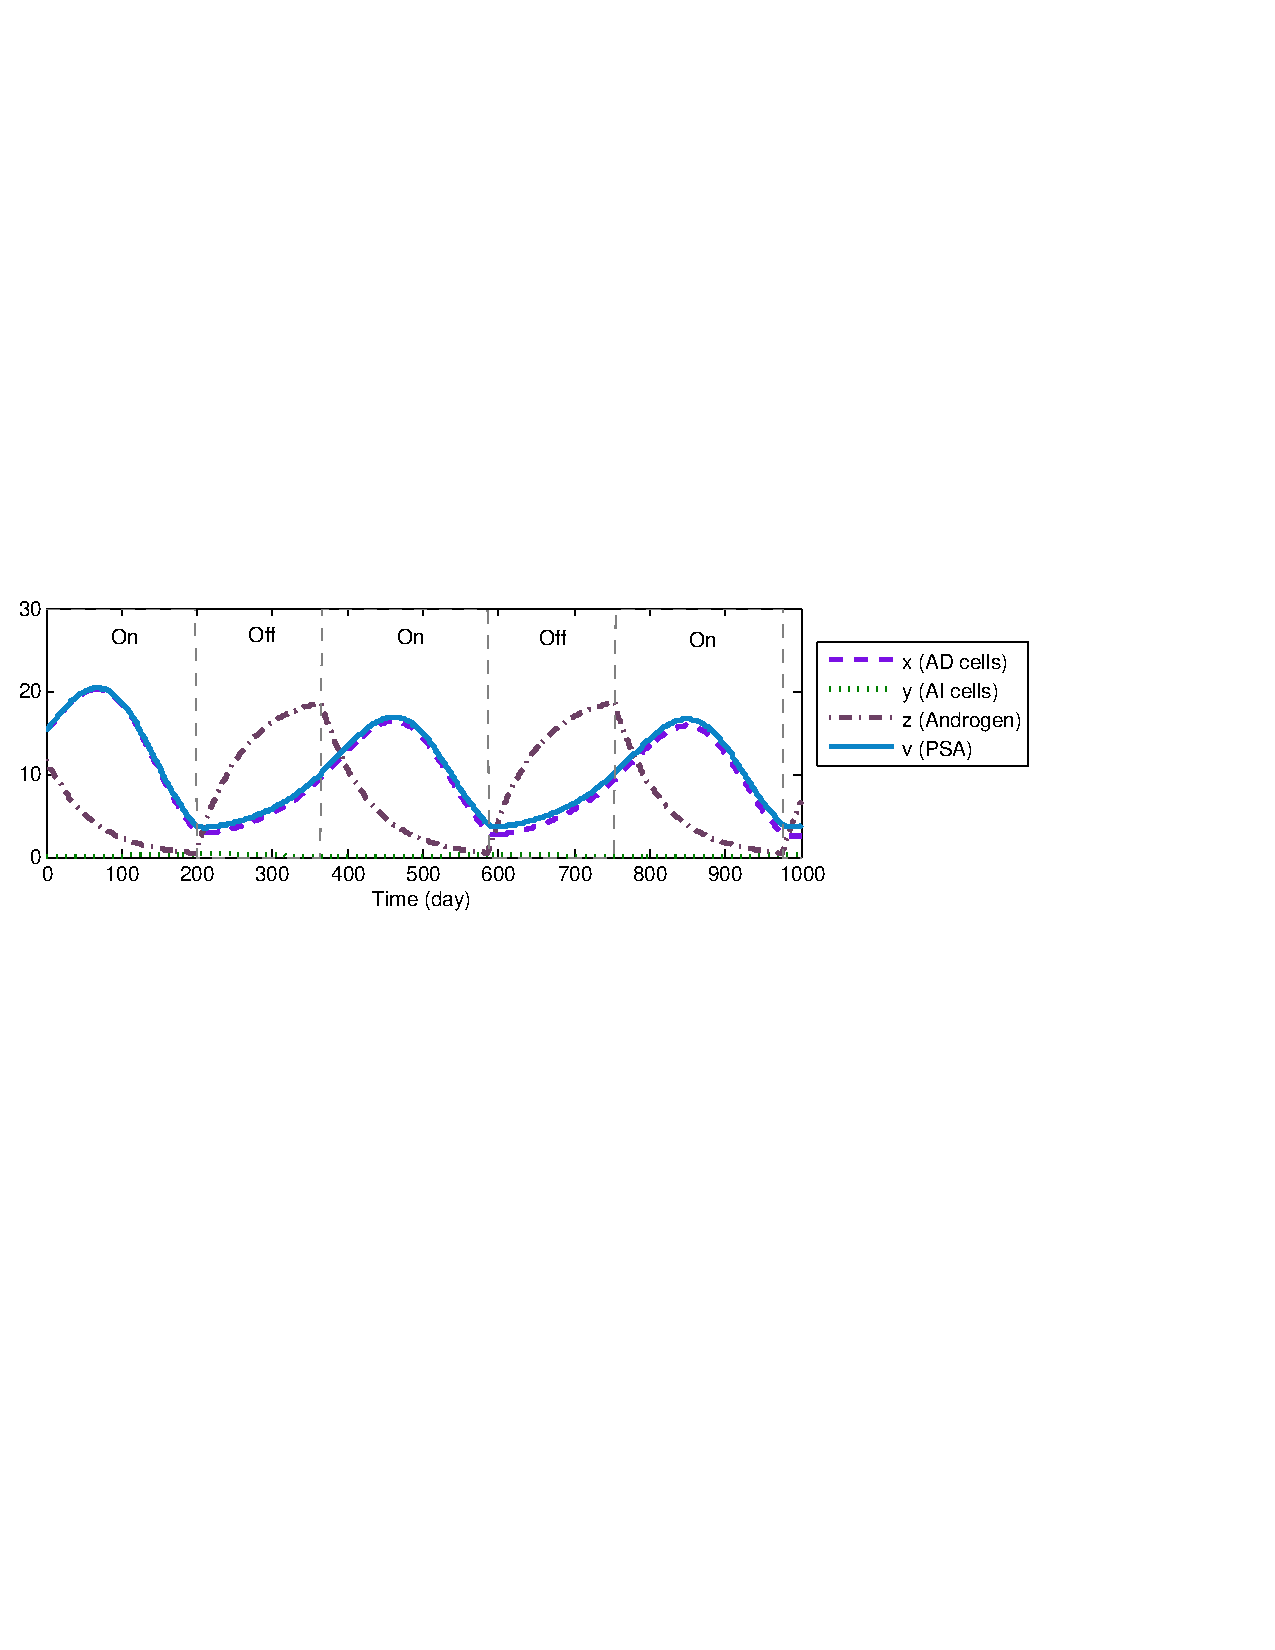
\includegraphics[scale=0.5]{fig-prostatetraj}
\caption{Simulated time profiles of $H_3$ model.}
\label{prostate-fig1}
 %\vspace{-0.7cm}
\end{figure}

\subsection{Androgen-dependent HSC dynamics}

As mentioned in Section \ref{sec.model}, previous studies \cite{jackson04a,jackson04b,ideta08} modeled the androgen-dependent proliferation and apoptosis of HSCs using MML functions, while we use sigmoid functions. Here we show that the MML based approach is unable to reproduce an important dynamical property, but our model could. The patients' data in \cite{ bruchovsky06,bruchovsky07} show that the \textit{half-time} $t_{1/2}$ (i.e. the amount of time required for a quantity to fall to half its initial value) of PSA level under androgen suppression is often less than $60$ days. To specify this property, we introduced an auxiliary mode (Mode 3). If $v(t)=v(0)/2$, the system will jump from Mode 1 to Mode 3. Starting with Mode 1 and $15 \le z(0) \le 17$, we checked reachability of a goal state with $0 \le w \le 60$ for both Ideta's model \cite{ideta08} and our model. The results show that  $\delta$-$\mathsf{sat}$ was return for our model, while $\mathsf{unsat}$ was returned for Ideta's model, suggesting the superiority of sigmoid functions over MML functions in capturing HSC dynamics.


% <--

\subsection{Personalized therapy design}
We next apply $\delta$-reachability analysis to design treatment scheme for individual patients. Note that the parameter values in Table \ref{prostate} are the baseline parameters. Among patients, the values of some parameters vary, which causes the variability in responsiveness to hormone therapy. We select a set of ``personalized parameters'' including $\alpha_y$ (the proliferation rate of HSCs), $\beta_y$ (the apoptosis rate of HSC cell), $m_1$ (the conversion rate from HSCs to CRCs), and $z(0)$ (normal androgen level). 

%The values of these parameters can be either experimentally measured \citep{berges95} or computationally determined from PSA time serials data \citep{hirata10}.



Figure \ref{patients}(a-c) illustrates the PSA dynamics of $3$ mock patients with different personalized parameters under the same IAS treatment scheme ($r_0=4$, $r_1=10$). IAS prevents the relapse for Patient A and delays the relapse for Patient B, but does not help Patient C. Figure \ref{patients}(d) shows that, by modifying the IAS scheduling parameters $r_0$ and $r_1$, the relapse of Patient C can be avoided or delayed. Thus, we can formulate the personalized therapy design problem as a parameter synthesis procedure: (i) fill in parameter values of a patient to $H_3$; (ii) set the ranges of scheduling parameters as $r_0 \in [0,8)$ (nM) and $r_1 \in [8,15]$; (iii) check if $H_3$ can reach a state with $t=1000$ given the ``no cancer relapse'' invariants. If $\mathsf{unsat}$ was returned, it means that androgen suppression therapy is not suitable for the patient. Otherwise, a treatment scheme containing feasible values of $r_0$ and $r_1$ will be returned, which could prevent or delay the relapse of the patient. Note that if $r_0=0$ is returned, it refers to the CAS scheme.

\begin{figure}[htb]
\centering
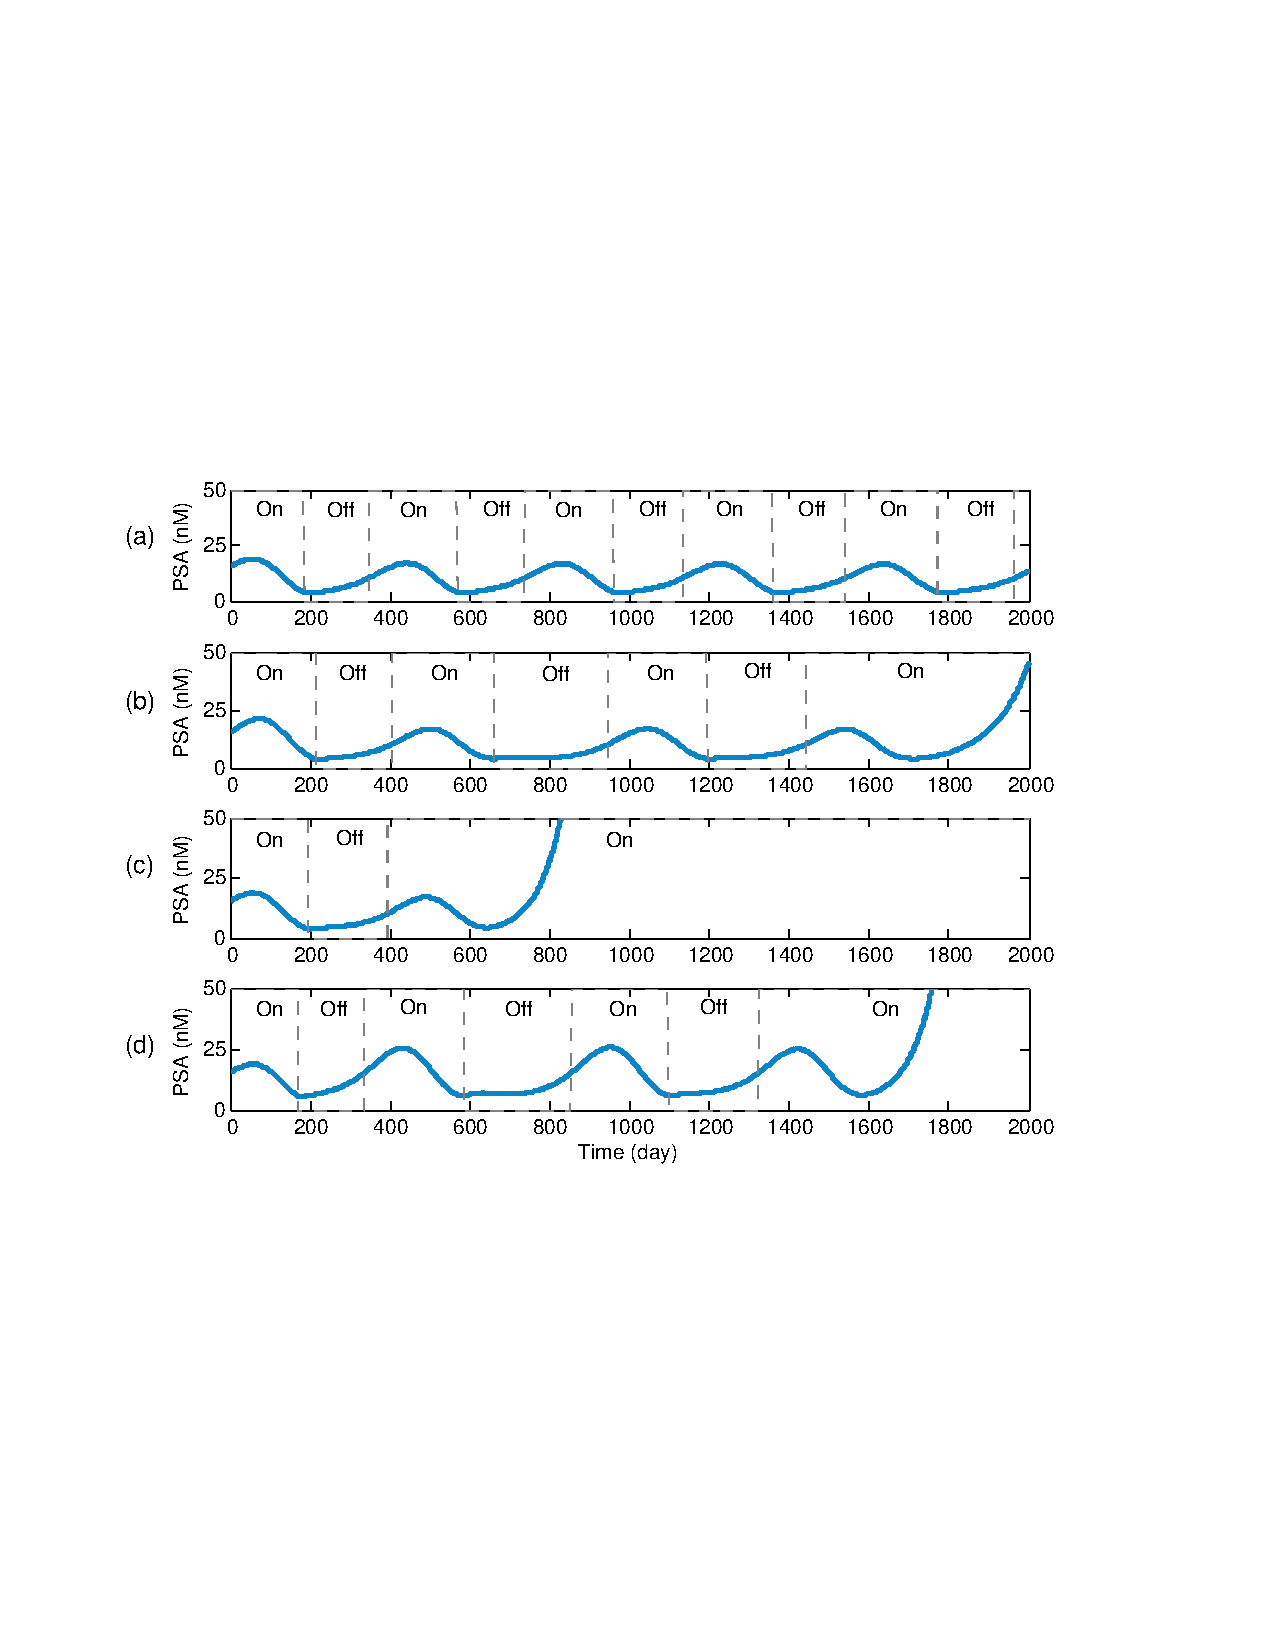
\includegraphics[scale=0.5]{fig-prostatetraj2}
\caption{Simulated PSA profiles of patients with different parameters. (a) Patient A: $\alpha_y=0.0242$, $\beta_y=0.0168$, $m_1=0.00005$, $z(0)=12$, $r_0=4$, $r_1=10$ (b) Patient B: $\alpha_y=0.24$, $\beta_y=0.13$, $z(0)=13$, $m_1=0.0001$, $r_0=4$, $r_1=10$ (c) Patient C: $\alpha_y=0.35$, $\beta_y=0.187$, $m_1=0.00005$, $z(0)=10$, $r_0=4$, $r_1=10$ (d) Patient C: $\alpha_y=0.035$, $\beta_y=0.187$, $m_1=0.00005$, $z(0)=10$, $r_0=6$, $r_1=15$.}
\label{patients}
 %\vspace{-0.7cm}
\end{figure}

We tested our method on real patients data collected by \cite{bruchovsky07}. The values of $\alpha_y$, $\beta_y$, $m_1$, and $z(0)$ for each selected patient were estimated by fitting the model to the PSA time serials data under the IAS therapy (data available at \verb#http://www.nicholasbruchovsky.com/clinicalResearch.html#). As an example, Figure \ref{fitting} shows the comparison between model predictions and the experimental data of PSA and androgen levels for Patient\#1. Table \ref{prostate2} summarized the suggested treatment scheme for selected patients. %The in silico validation results are shown in Supplementary Materials.

\begin{figure}[htb]
\centering
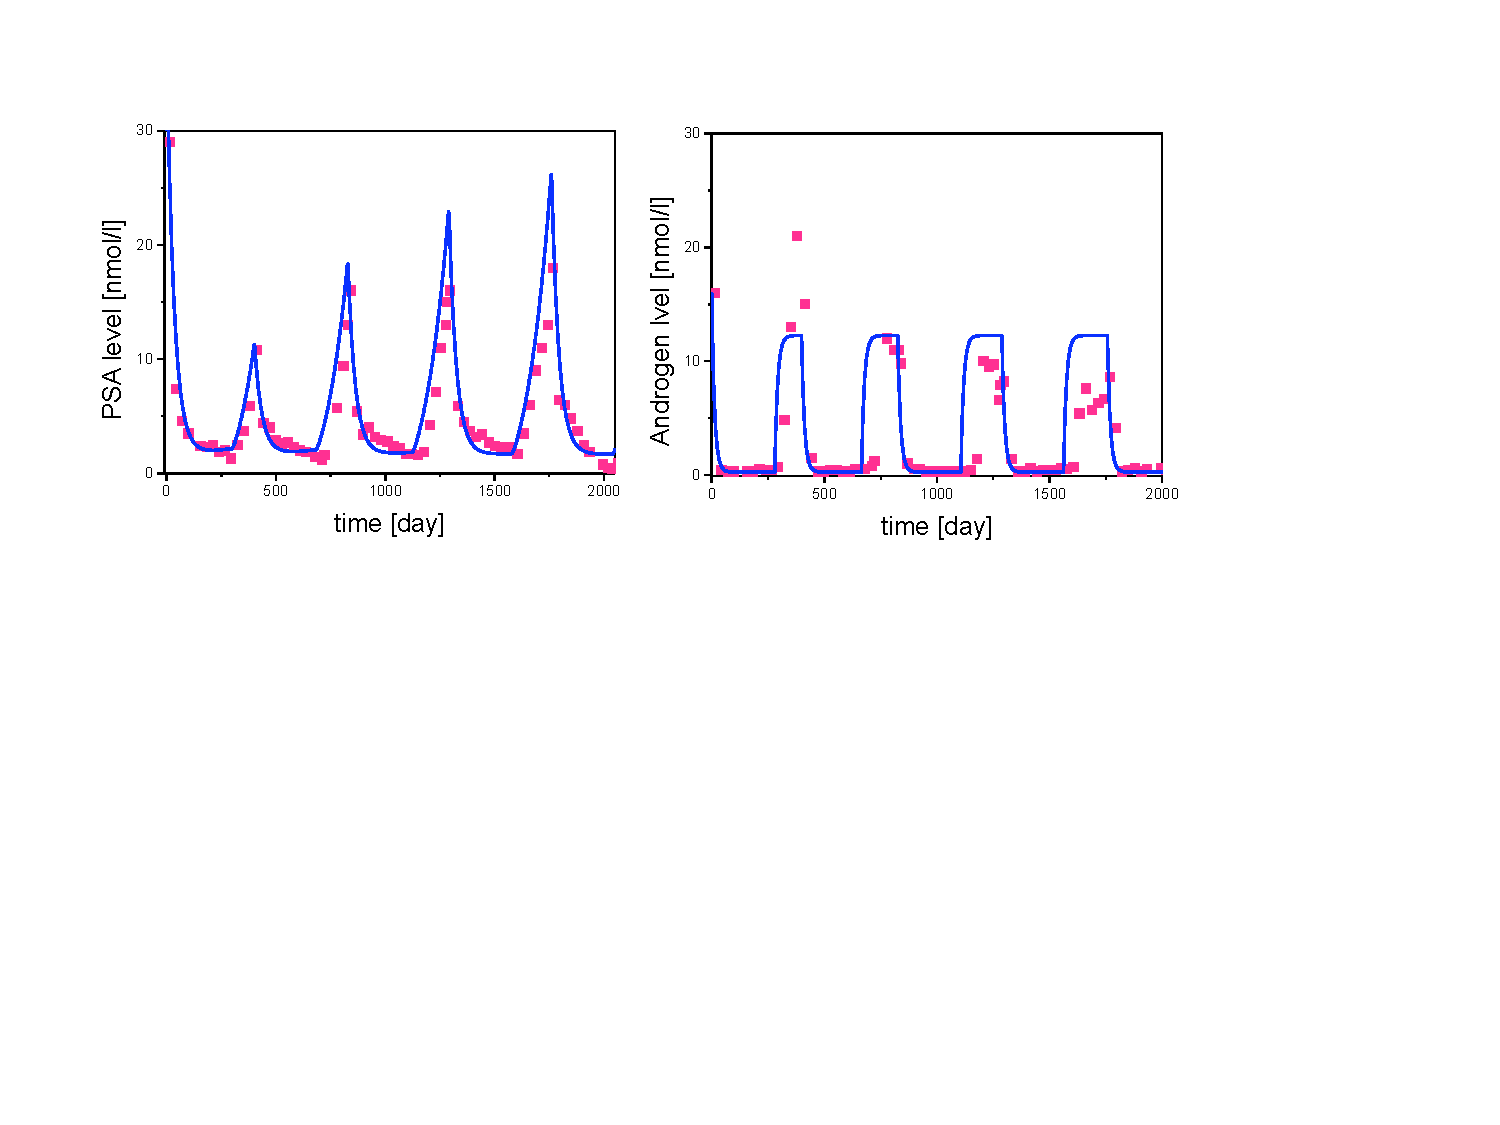
\includegraphics[scale=0.47]{fig-fitting}
\caption{Model prediction vs. experimental data.}
\label{fitting}
\vspace{-0.7cm}
\end{figure}


\begin{table}[h]
\caption{Predicted personalized therapy scheme\label{prostate2}}
\centering
\begin{tabular}{|c|c|}
\hline
Patient ID   & Suggested scheme  \\\hline
\#1 & $r_0=5.0$, $r_1=11.2$ \\
\#10 & $r_0=4.1$, $r_1=9.4$ \\
\#45 &  $r_0=3.8$, $r_1=12.2$ \\
\#97 &  N.A. \\
\hline
\end{tabular}
 %\vspace{-0.7cm}
\end{table}


%\begin{table}[h]
%\caption{Predicted personalized therapy scheme\label{prostate2}}
%\centering
%\begin{tabular}{c|c|c|c|c|c}
%\hline
%Patient ID  & $\alpha_y$  & $\beta_y$ & $m_1$ & $z(0)$ & Suggested scheme  \\\hline
%\#1 & 0.025 & 0.021  & 3.0E-5 & 8.23 & $r_0=5.0$, $r_1=11.2$ \\
%\#10 & 0.019 & 0.009  & 5.9E-5 & 9.44 & $r_0=4.1$, $r_1=9.4$ \\
%\#45 & 0.012  & 0.041  & 1.0E-5 & 12.61 & $r_0=3.8$, $r_1=12.2$ \\
%\#97 & 0.031  & 0.015  & 2.3E-5 & 10.61 & $-$ \\
%\hline
%\end{tabular}
% %\vspace{-0.7cm}
%\end{table}




